\documentclass[a4paper,11pt,uplatex]{jsarticle}


% 数式
\usepackage{amsmath,amsfonts}
\usepackage{bm}
\usepackage{physics}
% 画像
\usepackage[dvipdfmx]{graphicx}
\usepackage[dvipdfmx,colorlinks=true,linkcolor=blue]{hyperref}
\usepackage{pxjahyper}

\begin{document}


\section{実験装置}

\subsection{マインツマイクロトロン(MAMI)}
Mainz Microtron(MAMI)はドイツ、マインツ大学が所有する連続電子線加速器施設である。最大エネルギー1508 MeVの電子ビームを供給する
3台のRTM(Race Track Microtron)および1台のHDSM(Harmonic Double Siided Micrtron)から構成される。
ハイパー核生成実験ではHDSMを持ちいて最大エネルギーの1508 MeV
\subsubsection{電子ビームライン}
\subsubsection{ビーム調整}

\subsection{アンジュレータ}
\subsubsection{磁場制御}
マトリックス型のホールプローブを用いて磁場を測定する。
隣り合う電磁石の磁場が影響するため測定と電流のチューニングを繰り返し行う。
アンジュレータ通過後の電子ビームの方向のずれを最小に抑えることが重要となる。

\subsubsection{位置制御と読み取り}
可動範囲は 825 mm
ステップは 5 cm
モータ
(レーザを使った何か)で(um)単位で読み出す。

\subsection{分光光学系}
\subsubsection{スリット}
\subsubsection{grating}
\begin{itemize}
  \item フーリエ変換
  \item 分光
\end{itemize}

\subsubsection{波長分散レンズ}
\begin{figure}[tb]
  \centering
  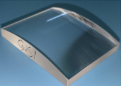
\includegraphics[width=0.8\linewidth]{image/3-lens.png}\\
  \caption{レンズ}
  \label{lens}
\end{figure}
\subsubsection{CMOS カメラ}

\subsection{分光光学系の較正}
波長較正として水銀灯を用いる。
$400 \text{nm}$領域には2本の輝線があり、このスペクトルを光学系で観測することで2つの輝線スペクトルを観測できる。
輝線スペクトルをガウス関数でフィッティングし、中心位置のピクセルを対応する波長にする。
2本のスペクトル以外のピクセルは2本の輝線の波長 -ピクセル関係の線形性を仮定して決定する。

\subsection{データ取得}
データの取得をスタートすると、指定された位置で4枚の写真を撮る。
露光時間は10 秒。
指定位置まで移動するとDAQに信号が送られ、DAQはカメラにシャッター信号を送信する。
\subsubsection{配線}

\subsection{電子ビーム測定}

ビームラインの切り替え\\
プロファイルモニタによるビームチューニング\\
画像によるビームチューニング\\

\subsection{}
\subsection{弾性散乱実験との接続}
\subsection{単アンジュレータによるデータ測定}

\clearpage

\begin{figure}[tb]
  \centering
  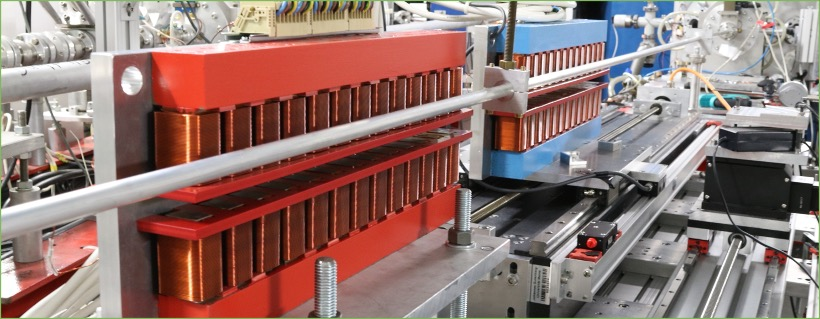
\includegraphics[width=0.8\linewidth]{image/1-1.jpg}\\
  \caption{サンプルの図}
  \label{sample_image}
\end{figure}

\begin{itemize}
  \item a
\end{itemize}
\begin{enumerate}
  \item b
\end{enumerate}

\begin{align}
\frac{1}{2} = \qty(\frac{1}{3}) + \qty{1}\Sigma
\end{align}
\end{document}